\documentclass[12pt,a4paper]{article}

% Compilação recomendada: pdflatex -interaction=nonstopmode PetCuida_documentacao.tex
\usepackage[utf8]{inputenc}
\usepackage[T1]{fontenc}
\usepackage[brazil, english]{babel} % Define os idiomas
\usepackage{lmodern}
\usepackage[a4paper,top=2.8cm,bottom=2.5cm,left=3cm,right=2cm]{geometry}
\usepackage{graphicx}
\usepackage{booktabs}
\usepackage{tabularx}
\usepackage{longtable}
\usepackage{array}
\usepackage{enumitem}
\usepackage{xcolor}
\usepackage{float}
\usepackage{caption}
\usepackage{hyperref}
\usepackage{microtype}
\usepackage{fancyhdr}
\usepackage{lastpage}

\definecolor{petgreen}{HTML}{2E7D5B}
\definecolor{petblue}{HTML}{256D85}
\definecolor{lightgreen}{HTML}{EEF7F2}
\hypersetup{colorlinks=true,linkcolor=petgreen,urlcolor=petblue,citecolor=petgreen,pdftitle={Documentação Final do Projeto PetCuida},pdfauthor={Grupo PetCuida}}
\setlength{\parindent}{1.25cm}
\setlength{\parskip}{0.25em}
\renewcommand{\arraystretch}{1.18}
\pagestyle{fancy}
\fancyhf{}
\lhead{PetCuida — Documentação final}
\rhead{Tópicos III}
\cfoot{\thepage\ de \pageref{LastPage}}
\newcolumntype{Y}{>{\raggedright\arraybackslash}X}
\newcommand{\todo}[1]{\textcolor{red}{[A preencher: #1]}}

\begin{document}
\selectlanguage{brazil}
\begin{titlepage}
\centering

\includegraphics[width=0.25\textwidth]{./images/brasao.png}\par
\vspace{0.5cm}
{\Large\textbf{PONTIFÍCIA UNIVERSIDADE CATÓLICA DE MINAS GERAIS}}\\[0.4cm]
{\large Curso de Engenharia de Computação}\\
{\large Disciplina: Tópicos III — Empreendedorismo e Inovação}\\
\vspace{0.5cm}
\IfFileExists{figuras/petcuida-logo.png}{
\includegraphics[width=0.28\textwidth]{figuras/petcuida-logo.png}\par\vspace{0.6cm}}{}
{\Huge\textcolor{petgreen}{\textbf{PetCuida}}}\\[0.4cm]
{\LARGE Documentação final do projeto}\\[0.7cm]
{\large Prevenção, créditos solidários e rede local de cuidado animal}

\vfill
\begin{tabular}{rl}
\textbf{Integrantes:} & Gabriel da Silva Cassino\\
 & Giovanna Naves Ribeiro\\
 & Júlia Rodrigues Vasconcellos Melo\\
 & Kathleen Rodrigues Leite Barbosa\\[0.3cm]
\textbf{Professor-orientador:} & João Carlos Oliveira Caetano\\
\textbf{Professor-tutor:} & Paulo Mattos
\end{tabular}

\vfill
Belo Horizonte\\2026
\end{titlepage}

\begin{abstract}
O PetCuida é uma plataforma mobile concebida para ampliar o acesso a cuidados veterinários preventivos e de menor custo. A solução reúne calendário de vacinação e vermifugação, prontuário digital, triagem orientativa não diagnóstica, rede local de prestadores e um mecanismo de créditos solidários. Este documento consolida a identificação e a validação do problema, a proposta de valor, a segmentação de clientes, o Business Model Canvas, o protótipo funcional, as estratégias de crescimento e escalabilidade e o plano de próximos passos. As evidências disponíveis indicam aderência inicial da solução às dores relatadas por tutores, mas permanecem exploratórias: os testes foram guiados, a amostra é pequena e ainda não há comprovação de receita, retenção ou disposição a pagar.
\end{abstract}

\textbf{Palavras-chave:} saúde animal; inovação social; plataforma bilateral; prevenção; créditos solidários; prototipagem.
\newpage

\selectlanguage{english}
\begin{abstract}
PetCuida is a mobile platform designed to expand access to preventive and lower-cost veterinary care. The solution integrates a vaccination and deworming schedule, digital medical records, non-diagnostic preliminary screening, a local network of service providers, and a "solidarity credits" mechanism. This document outlines the identification and validation of the problem, the value proposition, customer segmentation, the Business Model Canvas, a functional prototype, growth and scalability strategies, and a roadmap for next steps. Available evidence suggests an initial alignment between the solution and the pain points reported by pet owners; however, these findings remain exploratory—testing was conducted under controlled conditions, the sample size is small, and there is not yet any evidence regarding revenue, user retention, or willingness to pay.
\end{abstract}

\textbf{Keywords:} animal health; social innovation; two-sided platform; prevention; solidarity credits; prototyping.
\newpage

\selectlanguage{brazil}
\tableofcontents
\newpage

\section{Visão geral do projeto}
O PetCuida nasce da combinação de duas dificuldades recorrentes: o custo dos serviços veterinários e a ausência de ferramentas simples para organizar o cuidado preventivo. A proposta é conectar tutores, voluntários, organizações comunitárias e prestadores veterinários em uma rede local, na qual o cuidado possa ser planejado, acompanhado e parcialmente viabilizado por créditos obtidos em atividades solidárias.

A solução não pretende substituir consultas ou diagnósticos veterinários. A triagem é orientativa e deve encaminhar situações de risco para atendimento profissional. O produto encontra-se em estágio de validação inicial, com protótipo funcional em Flutter e evidências qualitativas de testes de usabilidade.

\begin{table}[H]
\centering
\caption{Resumo executivo do PetCuida.}
\begin{tabularx}{\textwidth}{>{\bfseries}p{3.4cm}Y}
\toprule
Problema & Tutores de baixa renda adiam cuidados, recorrem a fontes informais e perdem o histórico do animal.\\
Solução & Aplicativo de prevenção, orientação inicial, prontuário, rede solidária e encaminhamento local.\\
Público prioritário & Tutores das classes C, D e E, protetores/ONGs e prestadores veterinários regionais.\\
Diferencial & Combinação de prevenção, triagem não diagnóstica, créditos solidários, preço social e histórico digital.\\
Estágio & Protótipo funcional e validação exploratória; sem receita ou retenção comprovadas.\\
\bottomrule
\end{tabularx}
\end{table}

\section{Problema identificado e validação}
\subsection{Dor de mercado}
O cuidado com animais de estimação está presente em muitos lares, mas consultas, exames, vacinação e castração podem representar uma barreira severa para famílias com orçamento limitado. As entrevistas realizadas pelo grupo apontaram que o atendimento profissional frequentemente é tratado como último recurso. A prevenção é adiada, o calendário vacinal é esquecido e, diante de sintomas, alguns tutores procuram a internet, administram medicamentos por conta própria ou simplesmente aguardam uma melhora espontânea.

A dor também é operacional: a troca de profissionais e a ausência de um registro centralizado fazem com que o histórico médico do animal se perca. Em emergências, somam-se a distância até uma unidade disponível e a impossibilidade de comparar preços com calma. O resultado é um ciclo de atraso, agravamento do problema e aumento do custo.

\subsection{Entrevistas exploratórias}
Foram relatados oito depoimentos de tutores com perfis distintos. Os padrões mais relevantes foram:
\begin{itemize}[leftmargin=*]
  \item consultas e exames são percebidos como caros, sobretudo quando a situação já se tornou emergencial;
  \item vacinação e acompanhamento preventivo são irregulares ou dependem de campanhas públicas;
  \item há insegurança para decidir quando procurar atendimento e tendência a buscar orientação informal;
  \item animais resgatados e tutores de baixa renda têm forte vínculo afetivo, mas pouca capacidade de pagamento;
  \item a falta de atendimento 24 horas próximo agrava a vulnerabilidade em situações urgentes;
  \item há interesse em uma rede acessível, desde que exista confiança, orientação e divulgação local.
\end{itemize}

Uma formulação representativa da necessidade é: \textit{cuidar do animal com dignidade, mesmo quando o tutor não consegue pagar o preço integral de um atendimento particular}. A partir disso, o problema não é apenas localizar um prestador: envolve prevenção, orientação confiável, acesso financeiro e continuidade do cuidado.

\subsection{Testes de usabilidade e evidências}
O protótipo atual, denominado D4 (revisão interna \texttt{PetCuida\_D4C2B\_LGPD}), foi desenvolvido e disponibilizado ao longo de cinco revisões. Nas duas primeiras etapas, realizaram-se entrevistas para apresentar a proposta inicial, acompanhadas da transcrição integral dos diálogos e da identificação dos participantes, a fim de preparar as fases seguintes. Nas três revisões subsequentes, registraram-se apenas anotações dos pontos considerados relevantes, sem a identificação demográfica completa. Como a navegação foi conduzida pelos entrevistadores, o procedimento deve ser interpretado como uma demonstração guiada com coleta de feedback, e não como um teste autônomo de tarefas da aplicação.

Os resultados qualitativos obtidos foram majoritariamente favoráveis. A participante Aline comparou a experiência à de um aplicativo de mensagens e considerou a interface intuitiva. Já Galdina e Atanizia avaliaram a solução como interessante, mas destacaram a necessidade de maior divulgação. Outros relatos valorizaram funcionalidades específicas, como a triagem, os lembretes, a área dedicada ao pet, o prontuário e a centralização de diversas funções em um único ambiente.

Ressalta-se que a última versão conta com uma interface voltada para pessoa jurídica, desenvolvida ainda em estágio inicial e com margem para aprimoramentos. Adicionalmente, foi disponibilizado um formulário no Google Forms para a realização de uma pesquisa de mercado.


\begin{table}[H]
\centering
\caption{Principais achados da validação exploratória.}
\begin{tabularx}{\textwidth}{p{3.7cm}Y p{3.2cm}}
\toprule
\textbf{Achado} & \textbf{Interpretação} & \textbf{Situação}\\
\midrule
Facilidade percebida & Navegação principal considerada tranquila e familiar. & Confirmado qualitativamente\\
Triagem orientativa & Funcionalidade percebida como prática para decidir o próximo passo. & Manter e validar com supervisão técnica\\
Créditos solidários & Ideia compreendida parcialmente; faltou clareza sobre geração e uso. & Prioridade de melhoria\\
QR Code do prontuário & Finalidade não foi compreendida por uma participante. & Adicionar explicação contextual\\
Mapa e login & Ainda esquemáticos/simulados na versão alfa. & Integrações futuras\\
\bottomrule
\end{tabularx}
\end{table}

\subsection{Limitações da validação}
A amostra analisada é reduzida, não probabilística e parcialmente anônima. Em razão do baixo volume de dados coletados, não foram mensuradas métricas quantitativas de desempenho e negócio, como taxa de sucesso, tempo de execução de tarefas, frequência de erros, retenção, conversão ou disposição real de pagamento. Além disso, a coleta inicial ocorreu em um contexto informal, estando sujeita ao viés de cortesia devido à proximidade entre entrevistadores e participantes. Dessa forma, embora os resultados sustentem hipóteses iniciais de valor e usabilidade, eles não permitem generalizações para todo o público de tutores nem comprovam tração de mercado.

\section{Proposta de valor e segmentação}
\subsection{Proposta de valor}
A proposta central do projeto é: \textbf{``Cuidar antes, pagar de forma possível e encontrar orientação confiável: o PetCuida conecta tutores, serviços comunitários e prestadores veterinários em uma rede local de prevenção e cuidado acessível.''}

Para o tutor, o principal benefício é transformar o cuidado com o animal em uma rotina organizada, apoiada por lembretes, prontuário digital e orientação inicial. Quando houver necessidade de atendimento, a rede permite localizar parceiros, consultar preços sociais e combinar créditos da plataforma com pagamento monetário. Além disso, possibilita o incremento de renda por meio da prestação de serviços, caso o usuário deseje e esteja apto a realizá-los.

Para clínicas, veterinários e profissionais liberais, a plataforma atua como um canal para gerar demanda recorrente, ocupar horários ociosos e ampliar o alcance social de seus atendimentos. Por fim, para ONGs, instituições de ensino superior, protetores independentes e entidades similares, a solução potencializa o impacto social ao facilitar a oferta de atendimentos e serviços à comunidade.


\subsection{Diferenciais e salvaguardas}
\begin{enumerate}[leftmargin=*]
  \item \textbf{Prevenção ativa:} calendário de vacinação e vermifugação com lembretes.
  \item \textbf{Triagem não diagnóstica:} árvore orientativa para classificar urgência, agendamento ou observação, com encaminhamento profissional para sinais de risco.
  \item \textbf{Créditos solidários:} conversão de atividades comunitárias em saldo utilizável em serviços parceiros.
  \item \textbf{Prontuário digital:} histórico centralizado e exportável, evitando perda de informação.
  \item \textbf{Rede local:} curadoria de prestadores, preços sociais, reputação e campanhas comunitárias.
\end{enumerate}

A confiança depende de curadoria de parceiros, transparência de preços, regras auditáveis para os créditos, proteção de dados e linguagem explícita de que a triagem não substitui um médico-veterinário.

\subsection{Segmentos prioritários}
\begin{table}[H]
\centering
\caption{Segmentos, dores e valor entregue.}
\begin{tabularx}{\textwidth}{p{3.1cm}p{4.0cm}Y}
\toprule
\textbf{Segmento} & \textbf{Dores principais} & \textbf{Valor do PetCuida}\\
\midrule
Tutores de baixa renda & Custo, medo de emergências caras, falta de informação e prevenção. & Preços sociais, créditos, agendamento, lembretes e prontuário.\\
Tutores voluntários & Tempo disponível, mas pouco dinheiro para cuidar do próprio pet. & Troca de serviços por créditos veterinários.\\
ONGs e protetores & Muitos animais, recursos escassos e registros dispersos. & Rede, campanhas, voluntários e histórico centralizado.\\
Clínicas e veterinários & Agenda ociosa e baixa retenção local. & Novos clientes, ocupação e reputação de impacto social.\\
\bottomrule
\end{tabularx}
\end{table}

\section{Business Model Canvas}
O PetCuida opera como uma plataforma bilateral com camada solidária. O foco inicial deve ser hiperlocal, pois a troca só cria valor quando há densidade suficiente de tutores, voluntários e prestadores no mesmo território.

\begin{longtable}{p{3.4cm}p{11.2cm}}
\caption{Business Model Canvas do PetCuida.}\label{tab:bmc}\\
\toprule
\textbf{Bloco} & \textbf{Definição do modelo}\\
\midrule
\endfirsthead
\toprule\textbf{Bloco} & \textbf{Definição do modelo}\\\midrule
\endhead
Parcerias principais & Clínicas e veterinários regionais; ONGs e protetores; UBS Animal e secretarias; faculdades de Medicina Veterinária; pet shops, farmácias e laboratórios; fornecedores de nuvem e pagamentos.\\
Atividades-chave & Desenvolver e operar o app; credenciar prestadores; gerir créditos; manter protocolos; moderar a comunidade; educar preventivamente; proteger dados.\\
Proposta de valor & Prevenção, triagem orientativa, créditos solidários, preços transparentes, pagamento misto, prontuário único e ocupação de horários ociosos.\\
Relacionamento & Onboarding guiado; notificações; comunidade; suporte humano; avaliações mútuas; campanhas de vacinação e castração.\\
Segmentos & Tutores de baixa renda; tutores com tempo disponível; ONGs/protetores; clínicas e veterinários; pagadores institucionais.\\
Recursos-chave & App Flutter; Firebase; carteira de créditos; protocolos veterinários; base de prontuários; rede credenciada; equipe enxuta; marca comunitária.\\
Canais & Google Play; indicação em ONGs e grupos locais; QR codes em parceiros; eventos; redes sociais e conteúdo preventivo.\\
Estrutura de custos & Desenvolvimento; nuvem; consultoria veterinária; credenciamento; suporte/moderação; prevenção de fraude; marketing; pagamentos; LGPD.\\
Fontes de receita & Comissão de 8\%--12\% sobre dinheiro intermediado; PetCuida+; planos para clínicas; convênios e patrocínios; comissão de produtos parceiros. A troca de tempo permanece gratuita.\\
\bottomrule
\end{longtable}

A coerência do modelo está em monetizar os fluxos pagos, os serviços às clínicas e os convênios, preservando gratuitamente o núcleo de prevenção e a utilização dos créditos pelo público de baixa renda. Os principais riscos são liquidez local, adesão de prestadores, fraude, responsabilidade técnica e sustentabilidade do fundo de créditos.

\section{Protótipo e arquitetura da solução}
\subsection{Escopo funcional}
O protótipo desenvolvido em Flutter contempla as seguintes funcionalidades: autenticação, \textit{onboarding}, painel inicial, cadastro do pet, controle de vacinas, calendário, prontuário, geração de QR Code, triagem via questionário ou chat, rede solidária, mapa esquemático, agendamento, mural, perfil, gestão de saldo e suporte. Na versão alfa, os dados são armazenados localmente de forma simulada (\textit{mock}), e algumas integrações externas ainda operam em ambiente de simulação. Na revisão atual, incorporou-se um painel exclusivo para pessoas jurídicas, permitindo também o cadastro de seus respectivos funcionários.


\begin{figure}[H]
\centering
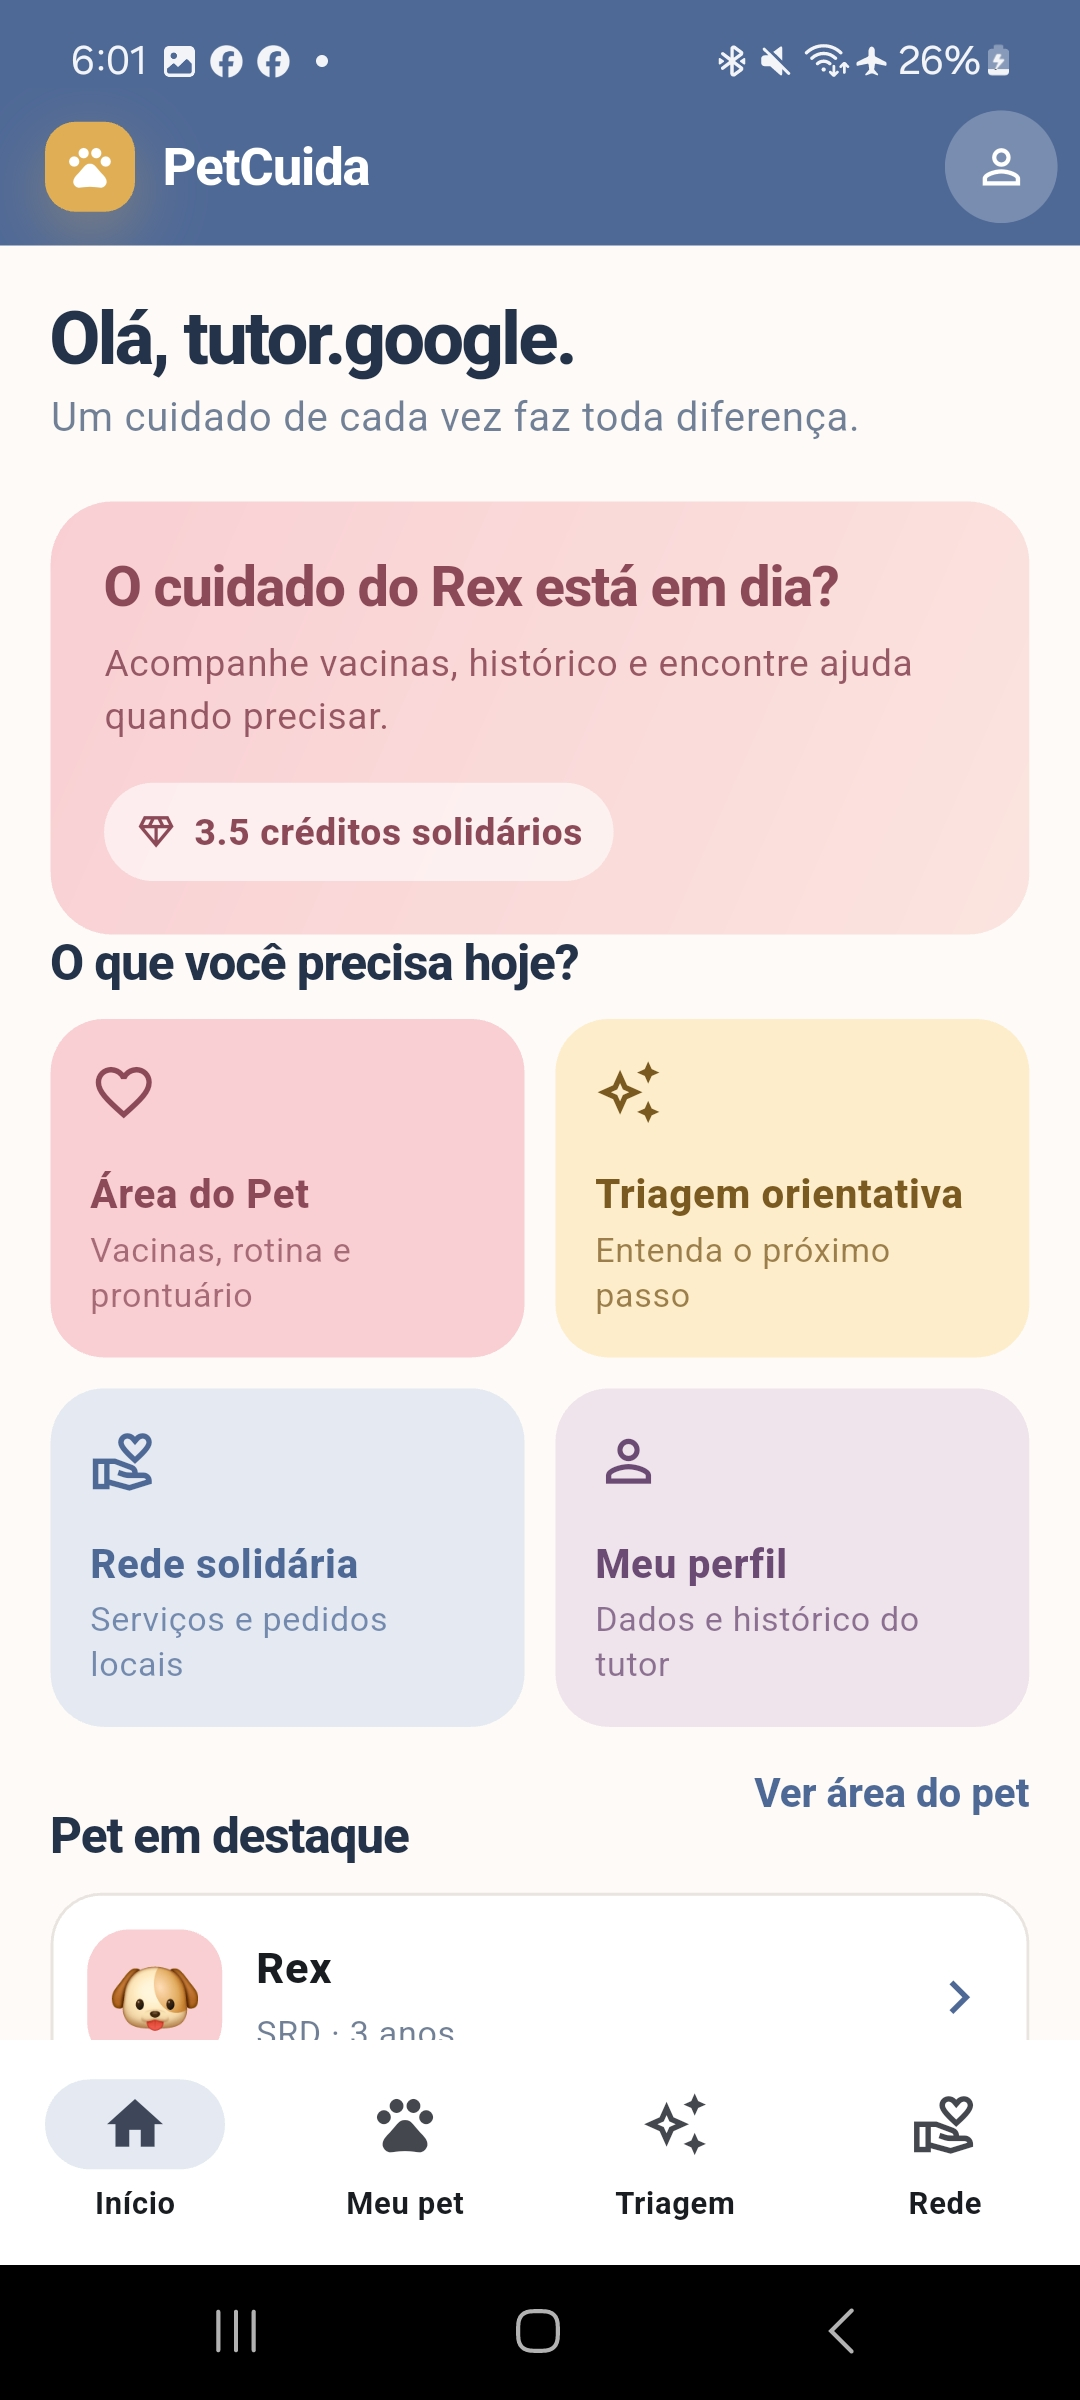
\includegraphics[width=0.38\textwidth]{figuras/homepage_v3e.jpg}
\caption{Painel inicial do protótipo PetCuida.}
\end{figure}

\begin{figure}[H]
\centering
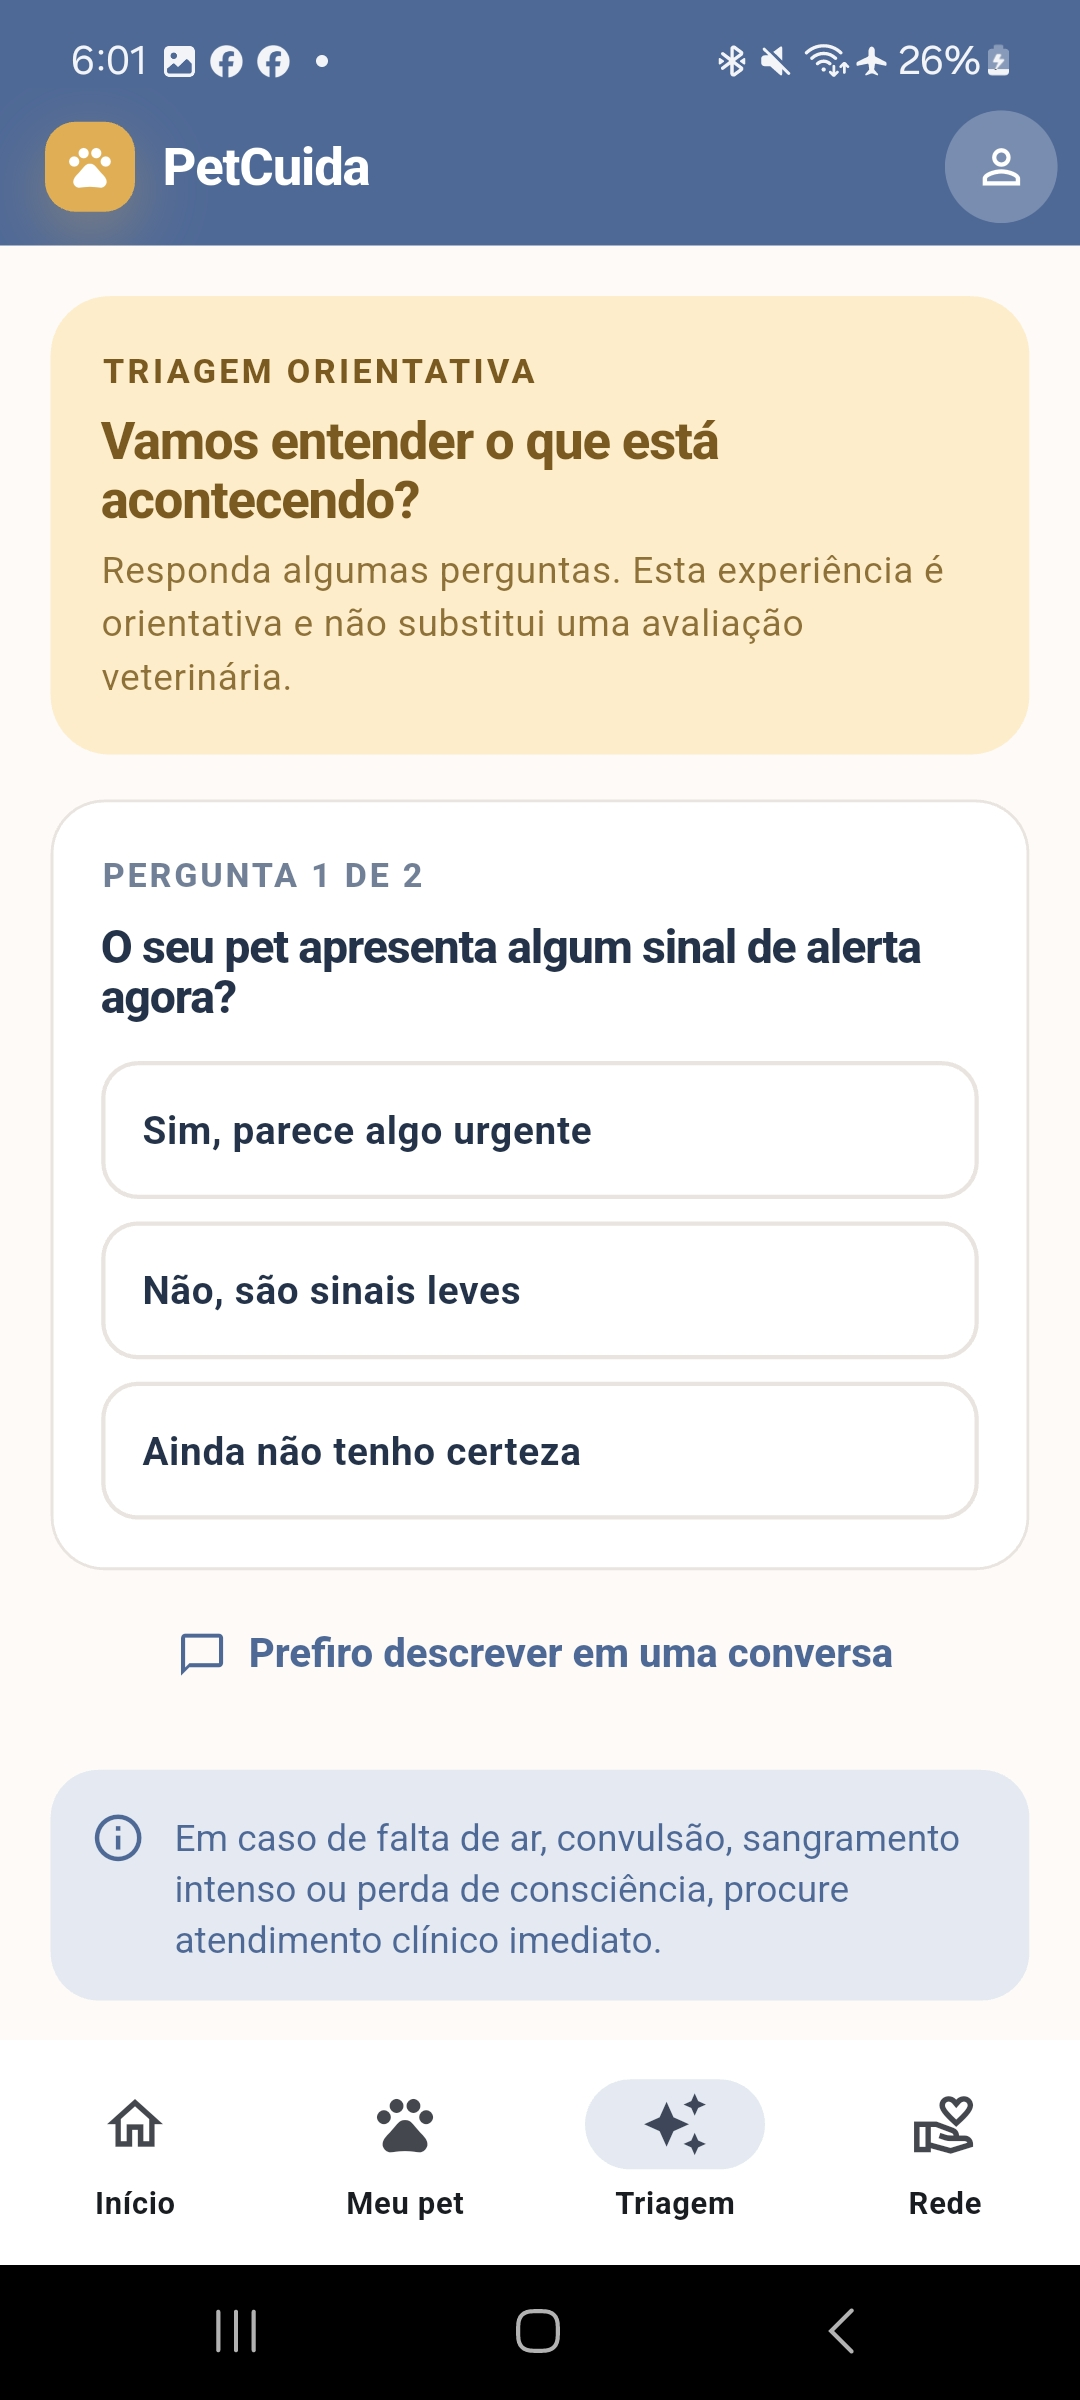
\includegraphics[width=0.38\textwidth]{figuras/triagem_v3e.jpg}
\caption{Fluxo de triagem orientativa.}
\end{figure}

\subsection{Arquitetura técnica registrada}
O projeto organiza o código por funcionalidades, com núcleo compartilhado:
\begin{verbatim}
lib/
  main.dart
  core/       theme, models, services, widgets, routes
  features/   auth, home, pet, triagem,
              rede_solidaria, perfil
\end{verbatim}

As decisões registradas incluem \texttt{provider} com \texttt{ChangeNotifier} para estado, \texttt{go\_router} para navegação e redirecionamento, \texttt{qr\_flutter} para o prontuário e fontes do sistema para manter o build leve. A compatibilidade declarada é Android 10 ou superior, com \texttt{minSdk 29} e \texttt{targetSdk 35}.

\begin{figure}[H]
\centering
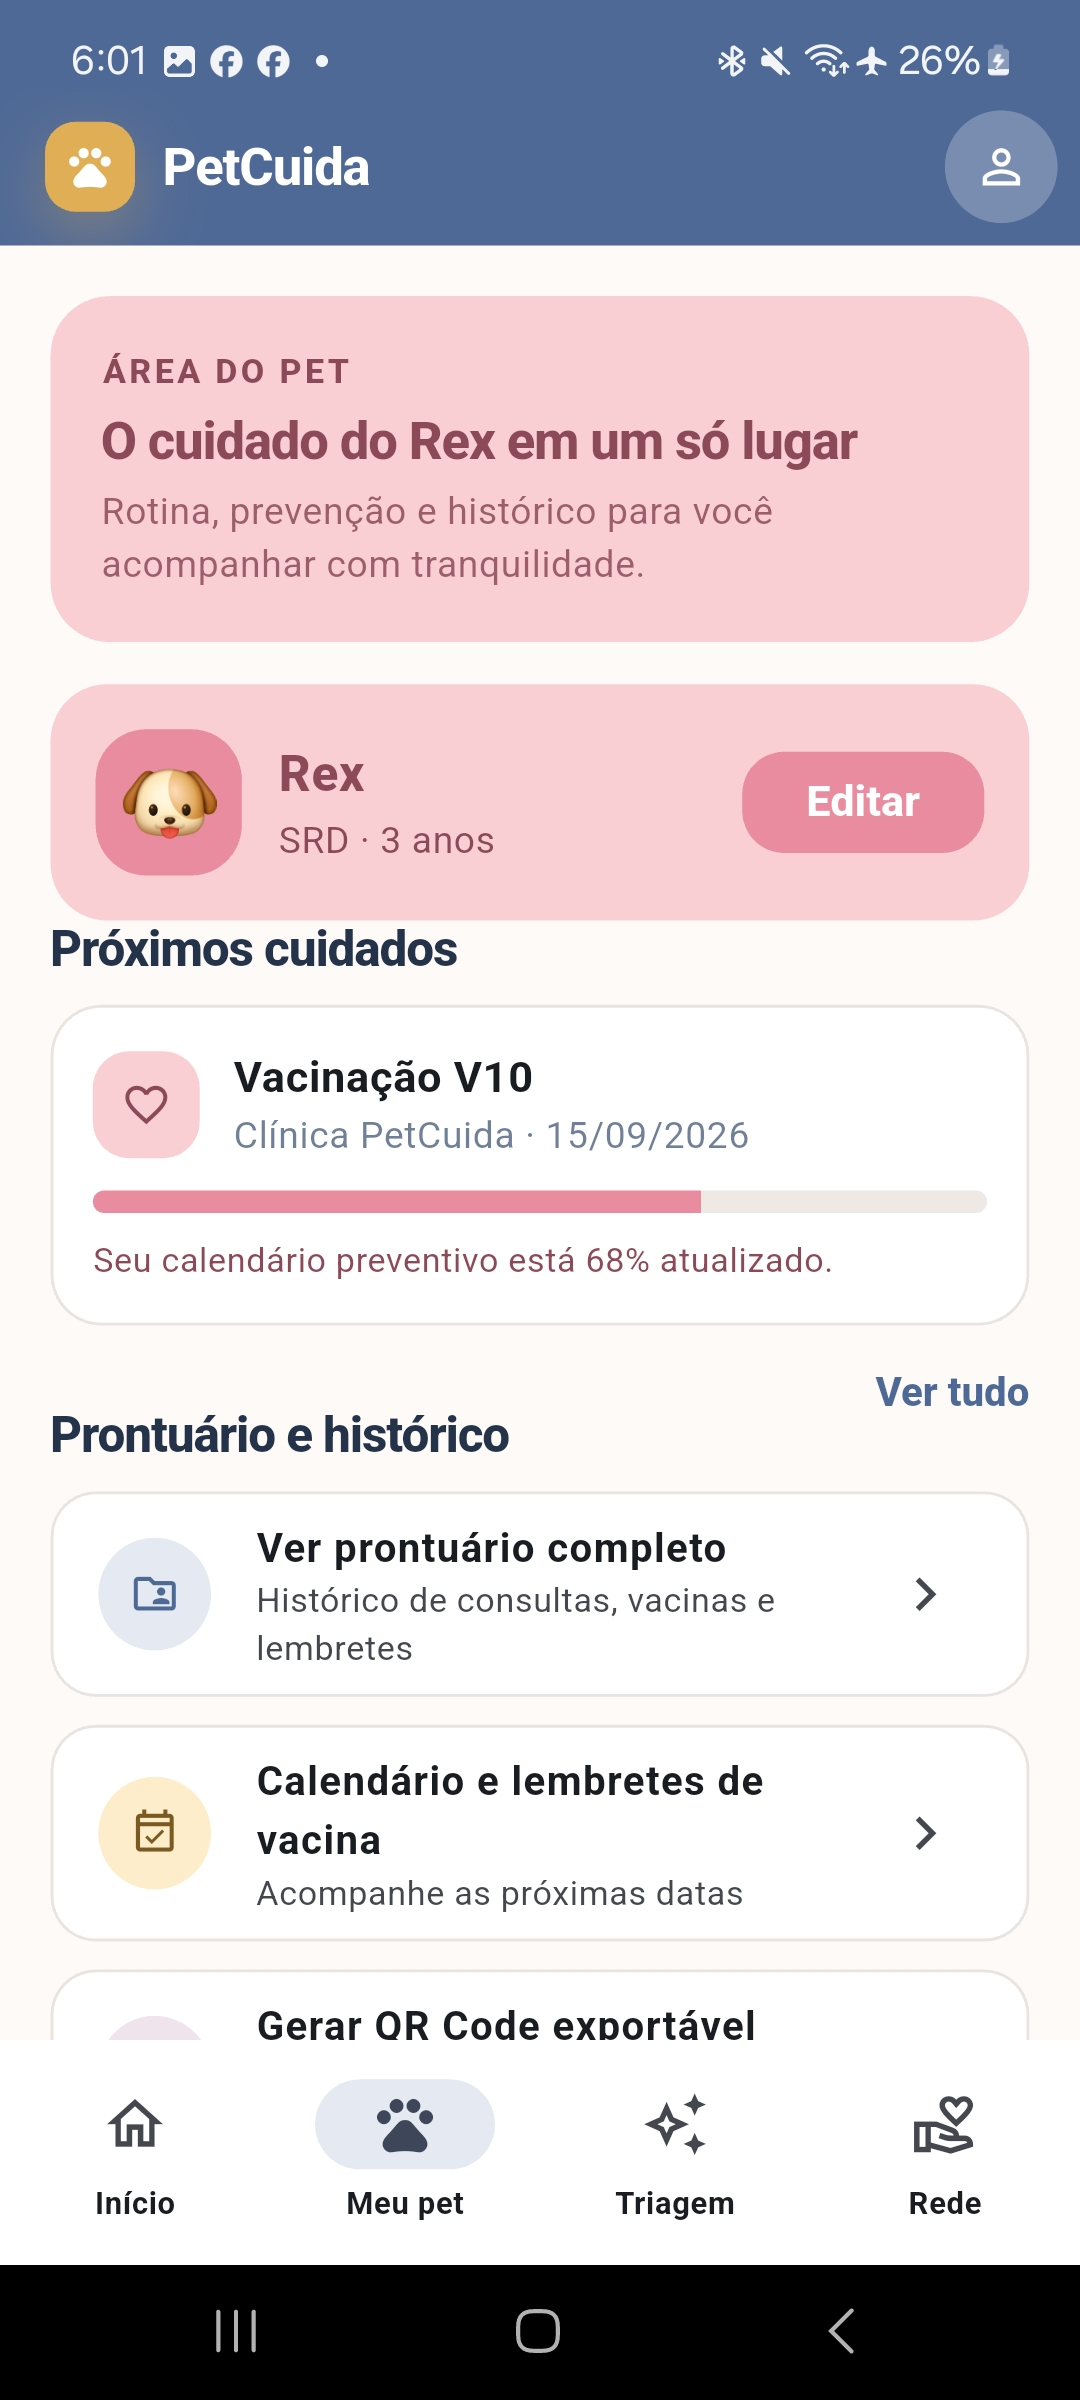
\includegraphics[width=0.42\textwidth]{figuras/pet_profile_v3e.jpg}
\caption{Área do pet com dados e histórico.}
\end{figure}

\subsection{Limitações técnicas atuais}
O mapa é esquemático; créditos, registros e login Google são demonstrativos; ainda faltam backend produtivo, pagamentos reais, notificações push, GPS, compartilhamento externo e controles completos de segurança. A triagem não realiza diagnóstico e deve permanecer subordinada a protocolos revisados por profissional habilitado.

\subsection{Aplicação web e API em Flask}
Além do aplicativo Flutter e da prévia estática, o pacote contempla uma implementação web completa em Python utilizando o microframework Flask, localizada no diretório \texttt{flask/}. A aplicação adota uma arquitetura desacoplada: o backend expõe rotas de API RESTful (definidas em \texttt{routes.py}), enquanto a interface do usuário é renderizada como uma \textit{Single Page Application} (SPA) reativa por meio de Vue.js (\texttt{vue.esm-browser.prod.js}) consumindo o cliente HTTP em \texttt{api.js}.

A estrutura funcional da versão Flask espelha e expande os fluxos do protótipo mobile, oferecendo autenticação, painel do tutor (\texttt{Dashboard.js}) e painel administrativo para pessoas jurídicas (\texttt{OrganizationDashboard.js}). Um diferencial relevante dessa implementação é a camada de abstração de persistência (\texttt{repository.py} e \texttt{data\_backends/}), que permite alternar entre armazenamento local ou bancos em nuvem por meio de adaptadores dedicados para Firebase Firestore e Supabase, além de incorporar controles explícitos de conformidade e anonimização previstos na Lei Geral de Proteção de Dados (\texttt{privacy.py} e \texttt{PRIVACIDADE\_LGPD.md}).

\begin{table}[H]
\centering
\caption{Principais módulos e arquivos da aplicação Flask recebidos no pacote.}
\begin{tabularx}{\textwidth}{p{4.5cm}Y}
\toprule
\textbf{Arquivo / Diretório} & \textbf{Função}\\
\midrule
\texttt{run.py} e \texttt{app/\_\_init\_\_.py} & Ponto de entrada da aplicação e inicialização da instância Flask.\\
\texttt{app/routes.py} & Definição dos \textit{endpoints} da API REST e renderização da página base.\\
\texttt{app/repository.py} e \texttt{db.py} & Camada de acesso a dados e gerenciamento de conexões.\\
\texttt{app/data\_backends/} & Adaptadores de persistência para Firestore e Supabase.\\
\texttt{app/privacy.py} & Regras de tratamento, consentimento e conformidade com a LGPD.\\
\texttt{app/static/js/components/} & Componentes Vue.js (\texttt{Login}, \texttt{Dashboard} e \texttt{OrganizationDashboard}).\\
\texttt{tests/} & Suíte de testes automatizados de rotas (\texttt{test\_app.py}) e privacidade (\texttt{test\_privacy.py}).\\
\bottomrule
\end{tabularx}
\end{table}

Para implantação em ambiente de produção, recomenda-se substituir o servidor de desenvolvimento do Flask por um servidor WSGI robusto (como Gunicorn ou uWSGI), configurar rigorosamente as variáveis de ambiente descritas em \texttt{.env.example}, ativar os adaptadores de banco de dados em nuvem com políticas de controle de acesso por perfil (PF/PJ) e executar continuamente a suíte de testes em \texttt{tests/} para assegurar a integridade das regras da LGPD.


\section{Estratégias de crescimento e escalabilidade}
\subsection{Diagnóstico do estágio}
A PetCuida está em validação inicial, antes da tração. Há protótipo e evidência exploratória de usabilidade, mas não há nos materiais analisados usuários pagantes, receita recorrente contratada, retenção medida ou contratos comerciais ativos. O setor pet é amplo, mas esse dado não substitui a validação de uma praça local.

\subsection{Estratégia 1 — Densidade local por parcerias}
A primeira estratégia é concentrar a operação em uma praça de Belo Horizonte, com duas ou três clínicas e até duas organizações comunitárias. A aquisição deve ocorrer por co-marketing, QR codes individualizados, indicação e eventos. O indicador não será download, mas cadastro ativado, encaminhamento concluído, retenção e oferta realmente disponível.

\subsection{Estratégia 2 — Aumentar contribuição por usuário}
A segunda estratégia testa a disposição a pagar por PetCuida+ e Plano Parceiro, além de patrocínios formais de campanhas. Esses serviços só devem ser ampliados após comprovação de demanda, conversão e margem. Intenção declarada não deve ser confundida com pagamento efetivo.

\subsection{Piloto assistido de oito semanas}
\begin{table}[H]
\centering
\caption{Plano do piloto territorial.}
\begin{tabularx}{\textwidth}{p{2.2cm}p{3.2cm}Y}
\toprule
Semanas & Foco & Entregas e evidências\\
\midrule
1--2 & Descoberta & 15--20 entrevistas; conversas com 5 clínicas e 2 organizações.\\
3--4 & Usabilidade & 10 testes autônomos, sem ajuda; taxa de conclusão, erros e dúvidas.\\
5--7 & Piloto concierge & Até 40--50 tutores e 2--3 clínicas, com acompanhamento manual e salvaguardas.\\
8 & Decisão & Continuar, iterar ou interromper com base em contagens, taxas e limitações.\\
\bottomrule
\end{tabularx}
\end{table}

Para escalar, a equipe deve primeiro padronizar processos e depois automatizá-los: onboarding de clínicas, QR codes, lembretes, indicadores, suporte e conciliação financeira. O “kit de praça” deve conter checklist, contrato revisado, critérios de credenciamento, materiais, treinamento, política de créditos e painel.

\section{Plano de próximos passos}
Para evoluir o protótipo atual (\texttt{D4C2B\_LGPD}) rumo a um piloto validado em ambiente real, estabeleceu-se um plano de ação dividido em frentes de usabilidade, engenharia, conformidade e validação de mercado:

\begin{enumerate}[leftmargin=*]
  \item \textbf{Refinamento de interface e fluxos:} Aprimorar a comunicação visual do sistema de créditos híbridos, inserir orientações contextuais sobre o uso do QR Code na própria tela e consolidar o painel para pessoas jurídicas (\textit{Organization Dashboard}).
  \item \textbf{Avaliação de usabilidade autônoma:} Conduzir uma nova rodada de testes sem mediação dos entrevistadores, mensurando taxas de conclusão e erros, além de aplicar um instrumento padronizado, como a escala SUS (\textit{System Usability Scale}).
  \item \textbf{Validação clínica e ética:} Revisar os fluxos de triagem orientativa junto a médicos-veterinários parceiros, garantindo a manutenção explícita de avisos de que a ferramenta não substitui o diagnóstico clínico presencial.
  \item \textbf{Governança e conformidade (LGPD):} Concluir a implementação dos requisitos previstos na documentação de privacidade do projeto, abrangendo gestão de consentimento, minimização de dados, controle de acesso por perfil (PF/PJ), políticas de retenção, rotinas de \textit{backup}, trilhas de auditoria (\textit{logs}) e plano de resposta a incidentes.
  \item \textbf{Integração de persistência em nuvem:} Substituir os dados locais simulados (\textit{mock}) pela ativação dos adaptadores de banco de dados em nuvem (Firestore ou Supabase) já estruturados na arquitetura do backend.
  \item \textbf{Operação piloto local:} Credenciar formalmente a primeira praça de operação, iniciando com duas a três clínicas veterinárias e organizações comunitárias (ONGs ou projetos universitários) para validar o fluxo real de atendimento.
  \item \textbf{Instrumentação de métricas:} Implementar a coleta de indicadores de produto e negócio, incluindo ativação (D7), retenção (D30), custo de aquisição de clientes (CAC) por canal, taxa de conversão paga, margem por atendimento e sustentabilidade do fundo de créditos.
  \item \textbf{Validação de monetização:} Testar a disposição real de pagamento por meio de pré-adesões, contratos piloto com parceiros ou transações reais, mantendo a distinção rigorosa entre projeções financeiras e resultados empíricos.
  \item \textbf{Documentação e governança da equipe:} Consolidar o manual de implantação em produção e revisar periodicamente a matriz de responsabilidades entre os integrantes a cada ciclo de desenvolvimento.
\end{enumerate}


\subsection{Equipe e governança}
A estrutura organizacional proposta busca ser funcional e enxuta, distribuindo as responsabilidades entre os integrantes da seguinte forma: Giovanna coordena a direção geral e a sustentabilidade financeira; Gabriel e Kathleen conduzem o desenvolvimento de produto e tecnologia; Kathleen também acompanha as operações e parcerias locais; e Júlia lidera as frentes de marketing, relacionamento, experiência do usuário e suporte. A governança operacional prevê reuniões semanais de acompanhamento, revisões quinzenais de produto, avaliações mensais de negócio e o registro contínuo das decisões tomadas.

Para orientar essas revisões e sustentar a tomada de decisão baseada em evidências, definiram-se os indicadores operacionais apresentados na Tabela~\ref{tab:indicadores}.

\begin{table}[H]
\centering
\caption{Indicadores e gatilhos de decisão.}
\label{tab:indicadores}
\begin{tabularx}{\textwidth}{p{3.8cm}Y}
\toprule
\textbf{Indicador} & \textbf{Definição operacional}\\
\midrule
Ativação D7 & Perfil do animal completo e ao menos um lembrete cadastrado em até sete dias.\\
Retenção D30 & Realização de ao menos uma ação de valor na plataforma entre os dias 22 e 30.\\
CAC ativado & Gastos atribuíveis ao canal divididos pelo total de usuários que atingiram a ativação D7.\\
Conversão paga & Assinantes pagantes ativos divididos pelos usuários ativos elegíveis, excluindo períodos de teste gratuito.\\
Margem por atendimento & Comissão recebida subtraída de taxas financeiras, impostos, custos variáveis e créditos liquidados.\\
\bottomrule
\end{tabularx}
\end{table}

A abertura de uma segunda praça de operação deve depender do cumprimento rigoroso dos seguintes critérios: dois ciclos mensais consecutivos com oferta contratada, coortes mensuráveis, CAC compatível com o retorno (\textit{payback}/CLV), margem unitária não negativa (ou subsídio formalmente contratado), receita efetivamente recebida e estabilidade operacional.

\section{Riscos, conformidade e limites}
A operação do PetCuida envolve desafios clínicos, financeiros, operacionais e regulatórios que exigem salvaguardas explícitas. A Tabela~\ref{tab:riscos} sintetiza os riscos prioritários mapeados e as respectivas estratégias de mitigação.

\begin{table}[H]
\centering
\caption{Matriz de riscos prioritários e ações de mitigação.}
\label{tab:riscos}
\begin{tabularx}{\textwidth}{p{4.2cm}Y}
\toprule
\textbf{Risco mapeado} & \textbf{Resposta e salvaguarda prevista}\\
\midrule
Interpretação da triagem como diagnóstico & Revisão de fluxos por médicos-veterinários e exibição permanente de avisos de caráter estritamente orientativo.\\
Fraude ou insuficiência do fundo de créditos & Regras auditáveis de emissão, limites de uso por usuário, lastro financeiro e conciliação periódica.\\
Baixa liquidez local & Foco hiperlocal na primeira praça e curadoria ativa de clínicas e organizações parceiras.\\
Privacidade e segurança da informação & Gestão de consentimento informado, minimização de dados, controle de acesso por perfil (PF/PJ) e trilhas de auditoria (\textit{logs}).\\
Atendimento manual excessivo & Padronização de processos via ``kit de praça'' antes da automação gradual de fluxos.\\
Baixa disposição a pagar e métricas infladas & Validação com transações reais e monitoramento de ativação (D7) e retenção (D30) em vez de apenas \textit{downloads}.\\
\bottomrule
\end{tabularx}
\end{table}

Em relação à conformidade legal, os dados pessoais dos tutores, os registros cadastrais de parceiros e o histórico clínico dos animais devem ser tratados em estrita observância à Lei Geral de Proteção de Dados (LGPD) e às diretrizes da Autoridade Nacional de Proteção de Dados (ANPD). Ressalta-se que, embora a arquitetura atual já contemple módulos iniciais de privacidade, a implantação produtiva integral dessas salvaguardas constitui requisito obrigatório antes da operação com usuários reais.

\section{Conclusão}
O PetCuida apresenta-se como uma resposta estruturada e coerente para uma dor validada qualitativamente: tutores de baixa renda necessitam de prevenção acessível, orientação inicial confiável e mecanismos financeiros viáveis, e não apenas de um catálogo de clínicas. O ecossistema prototipado — composto pelo aplicativo mobile em Flutter, pela aplicação web e API em Flask e pelos módulos iniciais de conformidade com a LGPD — integra funcionalidades reconhecidas como úteis pelos participantes, com destaque para a triagem orientativa, os lembretes preventivos, o prontuário digital e a rede solidária.

A principal conclusão estratégica deste ciclo é que a equipe deve comprovar a densidade local e a economia unitária antes de buscar escala ampla. O próximo passo prioritário não consiste em maximizar o volume de \textit{downloads}, mas em executar o piloto assistido de oito semanas, mensurar o comportamento real dos usuários, validar a disposição efetiva de pagamento, aprimorar a comunicação do sistema de créditos e consolidar uma rede confiável de oferta. Dessa forma, a expansão do projeto ocorrerá orientada por evidências empíricas, responsabilidade técnica e rigor na proteção de dados.

O grupo mantém a visão de que a prevenção, aliada à economia solidária, é um caminho promissor para democratizar o acesso à saúde veterinária no Brasil.

\appendix
\section{Links e materiais de referência}
\begin{itemize}[leftmargin=*]
  \item Repositório do projeto: \url{https://github.com/kasshinokun/Q3_Q4_2026_Public/tree/main/TOPICOS_III/}
  \item Pasta do protótipo e código: \url{https://github.com/kasshinokun/Q3_Q4_2026_Public/tree/main/TOPICOS_III/Atividade_VI}
  \item Aplicação web temporária indicada no README: \url{https://petcuida.pythonanywhere.com}
  \item Registro em vídeo dos testes: \url{https://youtu.be/uS83wGpVHdg}
\end{itemize}

\section{Fontes documentais utilizadas}
\begin{enumerate}[leftmargin=*]
  \item Atividade I-b — Identificação da dor de mercado e relatos de oito entrevistas, 2026.
  \item Atividade III — Business Model Canvas PetCuida, 2026.
  \item Atividade IV — Proposta de valor, segmentação de clientes e arquitetura de negócio, 2026.
  \item Atividade VI — Relatório de testes de usabilidade do aplicativo PetCuida Alpha 3i, 2026.
  \item Atividade XI — Estrutura organizacional e responsabilidades, 2026.
  \item Atividade XIII — Estratégias de crescimento, escalabilidade e viabilidade, 2026.
  \item Manual de Entrega 14 do Projeto — Documento final da disciplina, 2026.
\end{enumerate}

\end{document}
